\section{SWM với ánh xạ đặc trưng tuyến tính từng phần}
\subsection{Biên tuyến tính từng phần}
Trong vấn đề phân loại hai lớp, miền thường được phân chia thành hai phần bởi một biên, ví dụ như một siêu phẳng được tạo ra bởi các phương pháp phân loại tuyến tính, theo dữ liệu đầu vào \( x \in \mathbb{R}^n \) và nhãn tương ứng \( y \in \{+1, -1\} \). Các bộ phân loại tuyến tính đã được nghiên cứu trong nhiều năm, tuy nhiên, khả năng phân loại của chúng quá hạn chế và cần có các bộ phân loại phi tuyến. Trong đề án này, thuật ngữ khả năng phân loại của một bộ phân loại có nghĩa là tính linh hoạt của các loại và hình dạng có thể có của biên phân loại. Ví dụ, một bộ phân loại tuyến tính chỉ có thể cung cấp một biên tuyến tính, đó là một tập hợp affine, tức là một siêu phẳng, và do đó khả năng phân loại của nó không đủ cho nhiều ứng dụng. Theo một số quan điểm, mở rộng đơn giản nhất cho một tập hợp affine là một tập hợp tuyến tính từng phần, cung cấp một biên tuyến tính từng phần. Như tên gọi, một tập hợp tuyến tính từng phần bằng với một tập hợp affine trong mỗi vùng con của miền, và các vùng con phân chia miền.

\begin{figure}
    \centering
    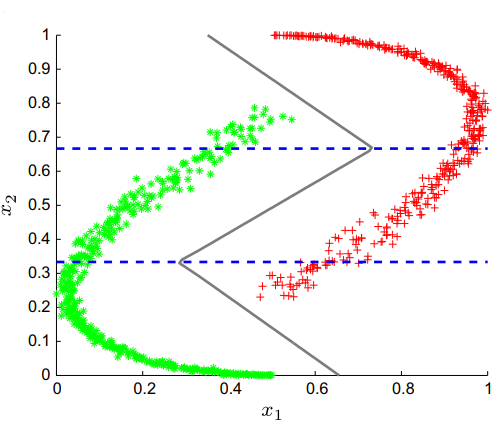
\includegraphics[width=0.73\textwidth]{images/moon_data.png}
    \caption[Tập dữ liệu hình mặt trăng]{\textbf{Tập dữ liệu hình mặt trăng}. Các điểm trong hai lớp được đánh dấu bằng các ngôi sao và các dấu chéo, tương ứng; ranh giới phân loại được hiển thị bằng các đường liền nét.}
    \label{fig:moon_data}
\end{figure}

Xét tập dữ liệu hai mặt trăng được hiển thị trong Hình \ref{fig:moon_data}, trong đó các điểm thuộc hai lớp được đánh dấu bằng các ngôi sao màu xanh lá cây và các dấu chéo màu đỏ. Hai lớp này không thể được phân tách bởi một biên tuyến tính và chúng ta có thể sử dụng một biên tuyến tính từng phần (PWL), được hiển thị bằng các đường màu đen, để phân loại hai tập dữ liệu này rất tốt. Tập hợp PWL này, được ký hiệu là \( \mathcal{B} \), bao gồm ba đoạn. Mỗi đoạn có thể được định nghĩa là một đường thẳng bị giới hạn trong một vùng con. Ví dụ, chúng ta có thể phân chia miền thành \( \om_1 = \{ x : 0 \leq x(2) \leq \frac{1}{3} \} \), \( \om_2 = \{ x : \frac{1}{3} \leq x(2) \leq \frac{2}{3} \} \), \( \om_3 = \{ x : \frac{2}{3} \leq x(2) \leq 1 \} \), trong đó \( x(i) \) là thành phần thứ \( i \) của \( x \). Sau đó, \( \mathcal{B} \) có thể được định nghĩa là
\[
\mathcal{B} = \bigcup_{k=1}^{3} \{ x : c_k^T x + d_k = 0, x \in O_k \},
\]
trong đó \( c_k \in \mathbb{R}^2 \), \( d_k \in \mathbb{R} \) định nghĩa đường thẳng trong mỗi vùng con, như được hiển thị trong Hình \ref{fig:pwl_boundary}.

Để thuận tiện cho việc diễn đạt, định nghĩa của tập hợp tuyến tính từng phần được đưa ra dưới đây.

\begin{define}
    Nếu một tập hợp $\mathcal{B}$ được định nghĩa trong miền \( \om \subseteq \mathbb{R}^n \) thỏa mãn hai điều kiện sau:
    \begin{enumerate}[label=(\roman*)]
        \item Miền $\om$ được phân chia thành các đa diện hữu hạn \( \om_1, \om_2, \ldots, \om_K \), tức là \( \om = \bigcup_{k=1}^{K} \om_k \) và \( \overset{\circ}{\om_k} \cap \overset{\circ}{\om_l}= \emptyset \), \( \forall k \neq l \), trong đó \( \overset{\circ}{\om_k} \) là phần trong của \( \om_k \).
        \item  Trong mỗi vùng con, \( \mathcal{B} \) bằng với một tập hợp tuyến tính, tức là với mỗi \( k \), tồn tại \( c_k \in \mathbb{R}^n \), \( d_k \in \mathbb{R} \) sao cho \( \mathcal{B} \cap \om_k = \{ x : c_k^T x + d_k = 0 \} \).
    \end{enumerate}
    \label{def:pwl_set}
\end{define}

\begin{figure}
    \centering
    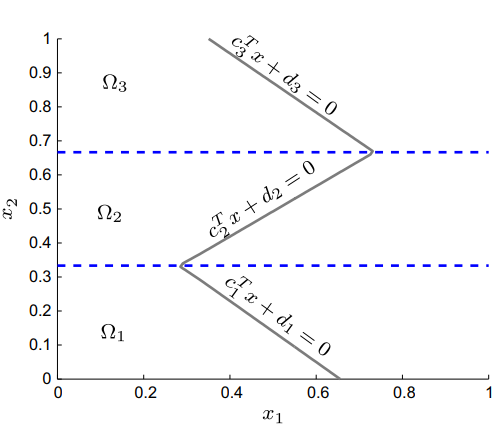
\includegraphics[width=0.7\textwidth]{images/pwl_boundary.png}
    \caption[Biên phân loại]{\textbf{Biên phân loại} bị giới hạn trong mỗi vùng con, ranh giới tuyến tính từng phần tương ứng với một đường thẳng.}
    \label{fig:pwl_boundary}
\end{figure}

Một tập hợp affine cung cấp một bộ phân loại tuyến tính, có thể được viết như là nghiệm của một phương trình tuyến tính \( f(x) = 0 \). Do đó, trong một vấn đề phân loại tuyến tính, người ta thường tìm kiếm một hàm tuyến tính \( f(x) \) để phân loại một điểm bằng dấu của giá trị hàm, tức là, \( \text{sign}\{f(x)\} \). Tương tự, một tập hợp \textbf{tuyến tính từng phần (PWL)} cung cấp một biên tuyến tính từng phần và nó có thể được biểu diễn như là tập nghiệm của một phương trình tuyến tính từng phần, được đảm bảo bởi định lý sau:

\begin{theorem}
    Mọi tập hợp tuyến tính từng phần \( \mathcal{B} \) đều có thể được biểu diễn như là nghiệm của một phương trình tuyến tính từng phần.
\end{theorem}

\begin{proof}
    Theo các ký hiệu trong Định nghĩa \ref{def:pwl_set}, giả sử số các đa diện xác định \( \mathcal{B} \) là \( K \) và các đa diện này được biểu diễn dưới dạng \( \om_k = \{ x : a_{ki}^T x + b_{ki} \leq 0, \forall 1 \leq i \leq I_k \} \), trong đó \( I_k \) là số các bất đẳng thức tuyến tính xác định \( \om_k \). Sau đó, ta xây dựng hàm sau:
    \begin{align}
        f(x) = \min_{1 \leq k \leq K} \left\{ \max \left\{|c_k^T x + d_k|, \max_{1 \leq i \leq I_k} \{ a_{ki}^T x + b_{ki} \} \right\} \right\}.
        \label{eq:pwl_function}
    \end{align}
    
    Vì hàm \( \max \) và hàm giá trị tuyệt đối đều liên tục và tuyến tính từng phần, ta có thể xác nhận rằng hàm \eqref{eq:pwl_function} là một hàm PWL liên tục. Tiếp theo, ta cần chứng minh rằng \( \mathcal{B} = \{ x : f(x) = 0 \} \).

    Đầu tiên, ta phải chứng minh \( \mathcal{B} \subseteq \{ x : f(x) = 0 \} \). Lấy một điểm tùy ý trong \( \mathcal{B} \), ký hiệu là \( x_0 \). Theo định nghĩa của tập hợp tuyến tính từng phần, ta có thể tìm một chỉ số \( k_0 \) sao cho \( x_0 \in \om_{k_0} \) và \( c_{k_0}^T x_0 + d_{k_0} = 0 \). Lại có
    \[
    \max_{1 \leq i \leq I_{k_0}} \{ a_{k_0i}^T x_0 + b_{k_0i} \} \leq 0,
    \]
    Do đó
    \[
        \max \left\{|c_k^T x + d_k|, \max_{1 \leq i \leq I_{k_0}} \{ a_{ki}^T x + b_{ki} \} \right\} = 0,
    \]
    trong đó \(I_{k_0}\) là số các ràng buộc xác định đa diện \(\om_{k_0}\). Vì \( \om_1, \om_2, \ldots, \om_K \) tạo thành một phân hoạch của miền nên \( \overset{\circ}{\om_k} \cap \overset{\circ}{\om_l}= \emptyset \), \( \forall k \neq l\). Do đó, \( x_0 \notin \overset{\circ}{\om_k} \), \( \forall k \neq k_0 \), tức là
    \[
    \max_{1 \leq i \leq I_k} \{ a_{ki}^T x_0 + b_{ki} \} \geq 0, \forall k \neq k_0,
    \]
    từ đó suy ra
    \begin{align*}
        \max &\left\{|c_k^T x_0 + d_k|, \max_{1 \leq i \leq I_k} \{ a_{ki}^T x_0 + b_{ki} \} \right\} \\
    &\geq \max \left\{|c_{k_0}^T x_0 + d_{k_0}|, \max_{1 \leq i \leq I_{k_0}} \{ a_{k_0i}^T x_0 + b_{k_0i} \} \right\} = 0,
    \end{align*}
    và
    \[
    f(x_0) = \max \left\{ |c_{k_0}^T x_0 + d_{k_0}|, \max_{1 \leq i \leq I_{k_0}} \{ a_{k_0i}^T x_0 + b_{k_0i} \} \right\} = 0 
    \]
    Suy ra \( \mathcal{B} \subseteq \{ x : f(x) = 0 \} \).

    Tiếp theo, ta chứng minh rằng \( \{ x : f(x) = 0 \} \subseteq B \). Giả sử \( x_0 \in \{ x : f(x) = 0 \} \),
    tức là \( f(x_0) = 0 \). Khi đó tồn tại ít nhất một chỉ số \( k_0 \in \{ 1, 2, \ldots, K \} \) sao cho
    \[
    \max \left\{ |c_{k_0}^T x_0 + d_{k_0}|, \max_{1 \leq i \leq I_{k_0}} \{ a_{k_0i}^T x_0 + b_{k_0i} \} \right\} = 0.
    \]
    Rõ ràng, \( c_{k_0}^T x_0 + d_{k_0} = 0 \) và \( a_{k_0i}^T x_0 + b_{k_0i} \leq 0, \forall 1 \leq i \leq I_{k_0} \), tức là \( x_0 \in \om_{k_0} \).
    Từ đó, có thể kết luận rằng \( x_0 \in \mathcal{B} \cap \om_{k_0} \subseteq \mathcal{B} \) và do đó
    \( \{ x : f(x) = 0 \} \subseteq \mathcal{B} \).

    Cuối cùng, ta được \( \mathcal{B} = \{ x : f(x) = 0 \} \), tức là bất kỳ tập hợp tuyến tính từng phần nào cũng có thể được biểu diễn như là tập nghiệm của một phương trình tuyến tính từng phần liên tục.
    \label{thm:pwl_set}
\end{proof}

\subsection{Phương trình tuyến tính từng phần}
Từ các công thức \sloppy \( |t| = \max\{t, -t\}\), \( \forall t \in \mathbb{R} \) và \( \max\{t_1, \max\{t_2, t_3\}\} = \max\{t_1, t_2, t_3\}\), \( \forall t_1, t_2, t_3 \in \mathbb{R} \), ta viết lại \eqref{eq:pwl_function} dưới dạng công thức min-max như sau:
\[
\min_{1 \leq k \leq K} \left\{ \max \{ c_k^T x + d_k, -c_k^T x - d_k, a_{k1}^T x + b_{k1}, \ldots, a_{kI_k}^T x + b_{kI_k} \} \right\}.
\]
Sử dụng công thức min-max, một bộ phân loại tuyến tính từng phần có thể được xây dựng. Vấn đề xác định các tham số có thể được đặt ra như một bài toán tối ưu không lồi và không khả vi của việc tối thiểu hóa hàm mất mát của các điểm bị phân loại sai. Tuy nhiên, vì bài toán tối ưu liên quan rất khó giải, số lượng các vùng con bị giới hạn ở một số nhỏ. Ví dụ, trong [8], chỉ các trường hợp với \( K \leq 5 \) được xem xét trong thí nghiệm số.
Để thu được các tham số một cách hiệu quả và đạt được khả năng tổng quát hóa tốt, trong đề án này, chúng tôi áp dụng kỹ thuật \textbf{Máy vector hỗ trợ (SVM)}. Để xây dựng một SVM mong muốn, ta cần một công thức khác được biến đổi từ \eqref{eq:pwl_function} dựa trên những điều sau:

\begin{lemma}[Định lý 1, Wang and Sun (18)]
    Cho hàm số \( f(x): \R^n \to \R \)
    \[
    f(x) = \max_{1 \leq k \leq K} \left\{ \min_{1 \leq i \leq I_k} \{ a_{ki}^T x + b_{ki} \} \right\}
    \]
    tồn tại \(M\) hàm cơ sở \( \phi_m(x) \) với các tham số \(\text{w}_m \in \R\), \(p_{mi} \in \R^n\) và \( q_{mi} \in \R \) sao cho
    \[
    f(x) = \displaystyle{\sum_{m=1}^{M}} \text{w}_m \phi_m(x),
    \]
    trong đó
    \[
    \phi_m(x) = \max \{ p_{m0}^T x + q_{m0}, p_{m1}^T x + q_{m1}, \ldots , p_{mn}^T x + q_{mn}\}.
    \]
    \label{lemma:wang_and_sun}
\end{lemma}

Theo Bổ đề \ref{lemma:wang_and_sun}, Định lý \ref{thm:pwl_set} và công thức \( \min_k\max_i\{t_{ik}\} = -\max_k\min_i\{-t_{ik}\}\), ta nhận được một công thức các hàm số tuyến tính từng phần khác. Kết quả này được mô tả trong Định lý sau đây, điều này làm cho SVM có thể áp dụng để xây dựng các bộ phân loại tuyến tính từng phần.

\begin{theorem}
    Mọi tập tuyến tính từng phần \(\mathcal{B}\) đều có thể được biểu diễn như là nghiệm của phương trình tuyến tính từng phần, tức là \(\mathcal{B} = \{x: f(x)=0\}\), trong đó, \(f(x)\) thỏa
    \begin{align}
        f(x)=\displaystyle{\sum_{m=1}^{M}} \text{w}_m \phi_m(x),
        \label{eq:pwl_f}
    \end{align}
    và 
    \begin{align}
        \phi_m(x) = \max \{ p_{m0}^T x + q_{m0}, p_{m1}^T x + q_{m1}, \ldots , p_{mn}^T x + q_{mn}\}.
        \label{eq:pwl_phi}
    \end{align}
    \label{thm:pwl_funtion}
\end{theorem}



